\documentclass{article} % For LaTeX2e
\usepackage{nips15submit_e,times}
\usepackage{hyperref}
\usepackage{url}
\usepackage{verbatim}
\usepackage{amsmath}
\usepackage{graphicx}
\DeclareMathOperator*{\argmax}{\arg\!\max}
\usepackage{multicol}
\usepackage{adjustbox}


\title{(T4-fMRI) Using fMRI to Diagnose Schizophrenia}
\author{
Farhad Haqiqat\\
Department of Computing Science\\
University of Alberta\\
\texttt{haqiqath@ualberta.ca} 
\And 
Neil Borle\\
Department of Computing Science\\
University of Alberta\\
\texttt{nborle@ualberta.ca}
\And 
Shashindra Silva\\
Department of Electrical and Computer Engineering\\
University of Alberta\\
\texttt{jayamuni@ualberta.ca}  
}
\newcommand{\fix}{\marginpar{FIX}}
\newcommand{\new}{\marginpar{NEW}}

\nipsfinalcopy 

\begin{document}

	\maketitle

\begin{abstract}
Diagnosing schizophrenia is a challenging task for which diagnostic tests
have yet to be developed, but where Functional Magnetic Resonance Imaging 
(fMRI) generated data is becoming increasingly available.
fMRI has been used in conjunction with Sparse 
Gaussian Markov Random Field (SGMRF) to achieve high accuracy when diagnosing
schizophrenia, however, these studies were limited by fairly small datasets
that originated from single locations. In this work we focus on obtaining
high diagnostic accuracies for data that has been combined from multiple
locations. We evaluated the performance of two main approaches. First, we 
used SGMRF classifiers on voxel degrees extracted from fMRI data. Second, we 
used Regions of Interest (ROI) defined by Power \emph{et al.} to extract a 
feature set from the data for learning and classification. 
After 5 repetitions of creating and evaluating on a balanced hold-out set where 
each location was represented equally, we found that an ROI approach used in 
conjunction with a SGMRF classifier provided the highest average accuracy 
($74.16\%$) on our multi-site 
data. While these accuracies are low in comparison to those obtain from
single site analysis, we show that reasonable accuracies can be obtain
when combining multiple schizophrenia datasets.
\end{abstract}


\section{Introduction}
Schizophrenia is a mental/psychiatric disorder~\cite{Rish_2013, Kenji_2010} 
known to affect blood flow in the brain~\cite{Kenji_2010} where those who are 
affected can experience hallucinations, delusions and diminished mental 
capacities to varying extents~\cite{jablensky2010diagnostic}. While several
features of schizophrenia have proven useful for its diagnosis there are
currently no set of features that have sufficient sensitivity or specificity
to be used in diagnostic tests~\cite{jablensky2010diagnostic, McGuire200891}. 
This effectively means that subjectivity plays a role when a physician is 
diagnosing a patient. 

Functional Magnetic Resonance Imaging (fMRI) is a tool for mapping of the 
functioning human brain caused by underlying brain electrical 
activity~\cite{fmriMatthews}. When a person is doing a task, neuron activity 
triggers increased blood flow to supply the neurons with 
the required glucose and oxygen\cite{fmriMatthews}. Increased blood flow also 
brings more oxygen through blood vessels. The change in the level of 
oxyhemoglobin and deoxyhemoglobin (oxygenated or deoxygenated blood) changes 
the magnetic susceptibility of blood (BOLD signal) which is detectable through 
fMRI~\cite{fmriMatthews}.

fMRI plays an important role in modern psychiatry research, as it provides the 
needed tool to determine dissimilarities in brain system that is a root for 
psychiatric illness\cite{Zhan_2015}. An advantage of fMRI is that it is 
non-invasive meaning that unlike some other imaging methods, no instruments or 
dyes are placed in the patient’s body~\cite{fmriMatthews, Grinvald_2000}. 

One of the tools used for studying schizophrenia is the
Sparse Gaussian Markov Random Field (SGMRF)~\cite{Rish_2013}\cite{Rosa_2013}. 
The primary advantage of using a SGMRF is that it has the ability to capture
inter-voxel relationships that other methods cannot~\cite{Rish_2013}.
The resulting relationships can be used to observe differences in functional 
connectivity in the brain, allowing healthy subjects to be differentiated from 
schizophrenic subjects. Automated approaches to schizophrenia
diagnosis have yielded accuracies of $93\%$ for data that 
originates from a single location~\cite{Rish_2013} and up to approximately 
$80\%$ for data that originates from multiple locations~\cite{Cheng2015}.

In this work we consider probabilistic graphical models (PGMs) as a means
of capturing differences in the interconnections between the brains of
healthy patients and the brains of schizophrenics. We compare several 
different methods including those that use voxel degrees, regions of 
interest, Markov network structure and several other features. 

\section{Background and Prior Work}

\subsection{Regions of Interest and Single-Voxel Analysis}
There are two main approaches for extracting
information from fMRI images. The first is a single-voxel approach and 
the second is to study regions of interest (ROI)~\cite{heller2006cluster}. 
The trade-off between these two approaches is that a single-voxel approach
requires the analysis of every voxel and is subject to the low signal-to-noise 
ratios of individual voxels, whereas a region based approach is only
effective if the selected regions capture all relevant information in an fMRI 
task~\cite{heller2006cluster}. In 2011, Power \emph{et al.} identified 264 
putative function regions of interest derived from resting state fMRI, where 
no specific task is performed during data collection~\cite{Power_2011}. 
JD Power argues that these regions are currently the best available 
representation of the functional networks in the brain~\cite{Power_2011}. 
Several of the approaches used in this study directly build upon these regions.


\subsubsection{Calculating Voxel Degrees}
Introduced as a ``degree map'' in Rish 
\emph{et al.}~\cite{rish2009discriminative}, voxel degrees are the constituent
components of degree maps and are a feature of fMRI data that has
been successfully used in schizophrenia diagnosis~\cite{Rish_2013}.
Voxel degrees represent the connectedness of voxels in the brain with the 
other voxels and are described as ``the number of voxel neighbours in a 
network''~\cite{Rish_2013}. Degrees are calculated in the following steps:
First, multiple pair-wise Pearson correlation comparisons between all voxels to 
create a correlation matrix. Second, a threshold is applied to the correlation
matrix. If a correlation value is greater than the threshold there said to be
an edge between those two voxels. Finally, all of the edges in which a voxel
participates are summed and the total number of edges becomes the 
degree of that voxel. Voxel degrees are used in several of our study's 
approaches.

\subsection{Rish \emph{et al.}}
Rish \emph{et al.}~\cite{Rish_2013} was able to achieve very high accuracies 
when diagnosing schizophrenia using fMRI data from a single location and 
employing several approaches. The most successful of these approaches include 
the use of support vector machines (SVM) and SGMRF classifiers, described 
later in the background. The error rate for SVM was 7\% using pairwise 
correlation features, and 14\% for the SGMRF using the $100$ most significant 
voxels in the degree map feature set. We use the SGMRF approach described by 
Rish \emph{et al.}~\cite{Rish_2013}. In the MRF classifier, first they split 
training data in two different groups. For each group they compute the 
precision matrix (assuming the data is centered unless $\mu$ needs to be 
computed as well). See the \textit{Inference} section of the Appendix for how 
they classify each new subject based parameters obtained from training stage.

%\begin{figure}
%  \begin{center}
%  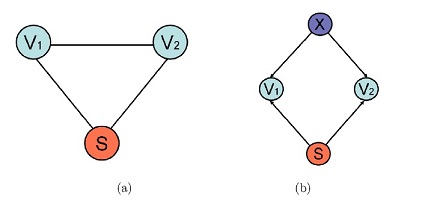
\includegraphics[width=0.5\textwidth, height=3.0cm]{diagrams/voxel.jpg}
%  \caption{Graphical models of voxel interactions Rish \emph{et al.}}
%  \label{voxel}
%  \end{center}
%\end{figure} 
%
%Figure \ref{voxel}.a shows interaction between voxels BOLD signal and a 
%stimulus, and Figure \ref{voxel}.b shows a Bayesian network of brain voxel 
%being affected by both stimulus and unobserved brain processes that can 
%change BOLD signal too. Given this figure one can see MRF approach invests 
%on the different network on of interaction for healthy versus schizophrenic 
%subject in response to a stimulus to differentiate them. 

\subsection{Rosa \emph{et al.}}
Work by Rosa \emph{et al.}~\cite{Rosa_2013} studied methods for diagnosing major 
depressive disorder (MDD). They used fMRI datasets and 
applied a SGMRF method to obtain the precision matrix. They then
use an SVM on the precision matrix for the classification task. 
They obtained 85\% accuracy on their first dataset and 78.95\% on their 
second dataset using this method. Both datasets were obtained using a single 
machine in a single location. The first dataset included $19$ patients 
and $19$ controls, and their second dataset included $30$ 
patients and $30$ controls. They also used SVM on the correlation feature, 
partial correlation and non sparse precision matrix to show effectiveness of 
their approach. Obtained accuracies were 68\% 53\% and 45\% respectively, 
which are all worse than sparse precision matrix. Their 
approach can be compared to our approach in the \textit{Individual MRF 
structure classification section}.       

\subsection{Multi-site Comparisons}
Although, there were several prior work on the classification of schizophrenia 
patients using fMRI, most are based on data from a single site. 
Classification from multi-site data is inherently difficult due to the batch 
effects resulting from the use of different machines and environments. At the 
same time, multi-site analysis can easily be generalized for a new data set 
from a totally different source. Cheng et al. \cite{Cheng2015} analyzes a 
multi site data set which is obtained from five different sites with different 
machines. They used SVM to classify schizophrenia patients and healthy 
controls, and obtained accuracies are in the range of $73.53- 80.92\%$. In this 
research we will try to obtain results with similar accuracies, but using PGM.


\subsection{Principal Component Analysis}
Principal Component Analysis (PCA) is a technique which uses 
mathematical techniques to transform data from an original space 
to a new dimensionality called principal components, which usually have 
smaller dimension than the original space. PCA uses vector 
space transformation to increase the dimensionality of large datasets. For 
doing so PCA uses mathematical projection~\cite{richardson2009principal}.

The way PCA does this projection is by maximizing the variance of projected 
data. As Bishop \cite{bishop2006pattern} shows, if we project the 
data on the eigenvector(s) of the data variance will be maximum. Hence, if we want 
to project our $N$-dimensional data to the $M$-dimensional space where $M<N$, 
\textit{"the optimal linear projection for which the variance of the 
projected data is maximized is now defined by the $M$ eigenvectors 
$u_{1}, ... , u_{M}$ of the data covariance matrix $S$ corresponding to the
$M$ largest eigenvalues $\lambda_{1}, ... ,\lambda_{M}$."}~\cite{bishop2006pattern}: 
$S$ and $\mu$ (the sample set mean) are defined as:

\begin{multicols}{2}
\begin{equation}
S = \frac{1}{N} \sum_{n=1}^{N}(X_{n}-\mu)(X_{n}-\mu)^T
\end{equation}\break
\begin{equation}
\mu = \frac{1}{N} \sum_{n=1}^{N}X_{n}
\end{equation}
\end{multicols}


\subsection{Support Vector Machines}
Vapnik \emph{et al.} introduced the concept of support 
Vector Machines (SVMs) as a statistical tool for 
classification problems~\cite{shmilovici2005support}. We
use the most simple SVM, a linear SVM, because it does not use non-linear
kernels and therefore has no hyperparameters that need to be tuned
with cross validation. Instead, a linear SVM learns the ``maximum-margin
hyperplane'' classifier which is a linear combination of the input 
features and partitions the data space into separate classes. The term 
``maximum-margin'' refers to the SVM's ability to find the maximal 
separation between classes and the hyperplane, therefore creating the 
largest ``margin''~\cite{shmilovici2005support}. We can be guaranteed of
the optimality of the result as the SVM problem is known to be 
convex~\cite{burges1998tutorial}. The most simple form of a linear SVM 
minimizes $\frac{1}{2}||w||^2$ subject to the constraint 
$y_i (x_i w + b) - 1 \ge 0 $, $\forall i$ where $w$ is the weight vector,
$x_i$ is the instance's features, $y_i$ is the instance label and $b$ is
the bias term of the model. Unfortunately, this version of the SVM only
works in cases where the data is linearly separable. To extend the SVM
to linearly inseparable data, the addition of positive slack variables is
required, such that the constraints become $\forall i$
$y_i (x_i w + b) - 1 + \xi_i \ge 0 $ and $\xi_i \ge 0$, where $\xi_i$ is 
the slack variable for the instance $i$~\cite{burges1998tutorial}.


\subsection{Sparse Gaussian Markove Random Field (SGMRF)}
One variation of Markov Random Field (MRF) is Gaussian MRF which is 
used for continuous space of variables and has well-defined mathematical 
properties that can be computed. Multivariate Gaussian density function 
over a set of random variables X is defined as below: 

\begin{equation}\label{gaussian1}
p(X) = (2\pi)^{-n/2} |\Sigma|^{-1/2} \exp\left\{ -\frac{1}{2}(X - \mu)^t \Sigma^{-1} (X - \mu) \right\}.
\end{equation}
 
In the equation $\mu$ is the mean and $\Sigma$ is the covariance matrix. 
We can set $\mu$ to zero and replace $\Sigma^{-1}$ with $C$ the 
equation \eqref{gaussian1} which can be written as the following form. 
It should also be noted that $C = \Sigma^{-1}$ and is known as the 
precision matrix in the literature.  

\begin{equation}\label{gaussian2}
p(X) = (2\pi)^{-n/2} |C|^{1/2} \exp\left\{ -\frac{1}{2}X^t C X \right\}.
\end{equation}

It has been shown by Lauritzen \cite{lauritzen1996graphical} that $X_i$ and $X_j$ are 
independent if and only if their corresponding entries in the precision 
matrix (C) are zero. It can be concluded that missing edge in the MRF will 
lead to zero entries in the precision matrix \cite{Rish2014Book}. The problem 
of learning pgm for a given dataset is reduced to 
learning the precision matrix given this proof.

The log-likelihood of the dataset, assuming each row of the data is a
p-dimensional vector and consisting n samples $D = \{X_1, X_2, ... , X_n\}$, 
can be written as follow. It should also be noted that we assume each sample 
is identically independent distributed (iid).

\begin{equation}
L(D) = \frac{n}{2} |C| - \frac{1}{2} \sum_{i=1}^{n} (X_i - \mu )^T C (X_i - \mu ) + const,
\end{equation}  

Here, \textit{const} is a constant which is not dependent on $\mu$ or $C$. We can also 
center the data in such a way that $\mu = 0$, so the second term reduces to 
$\frac{1}{2} \sum_{i=1}^{n} X_i ^T C X_i$ which is equal to 
$\frac{n}{2}$ tr($AC$), where $tr$ is trace of the matrix. The above 
formula can be written as shown in equation~\eqref{likelihood} where the
log-likelihood maximization problem is shown in 
equation~\eqref{maxlikelihood}. 

\begin{multicols}{2}
\begin{equation}\label{likelihood}
L(D) = \frac{n}{2} [|C| -  |tr(AC)|] + const
\end{equation}\break
\begin{equation}\label{maxlikelihood}
\max_{C\succ0} |C| - tr(AC)
\end{equation}
\end{multicols}

Here $|...|$ represents determinant and A is the empirical covariance 
matrix calculated by $A = \frac{n}{2} \sum_{i=1}^{n} X_i^T X_i$, or 
maximum likelihood estimation fo $\Sigma$. It should also be noted 
the $C\succ0$ constraint makes C positive definite.\\

To achieve sparse formulation for Gaussian Markov Random Field we can use 
the Laplace prior. If we impose the Laplace prior on the precision matrix 
$p(C_{ij}) = \frac{\lambda_{ij}}{2} e^{-\lambda_{ij}|C_{ij}|} $ we can 
achieve sparsity. This will change the equations \eqref{likelihood} and 
\eqref{maxlikelihood} to the following forms below where the $l_{1}$-norm 
of $C$ is $||C||_{1}= \sum_{ij}C_{ij}$, and $\rho=\frac{n}{2}\lambda$.

\begin{multicols}{2}
\begin{equation}\label{loglikelihood}
L(D) = \frac{n}{2} [ln|C| -  |tr(AC)|] - \lambda||C||_{1}, 
\end{equation}\break
\begin{equation}\label{logmaxlikelihood}
\max_{C\succ0} ln|C| - tr(AC) - \rho||C||_{1},
\end{equation}
\end{multicols}


\subsubsection{Method for obtaining precision matrix}  
One obvious way for learning the parameters for joint distribution probability 
is using regularized likelihood maximization such as Akaike information criterion (AIC) and Bayesian information criterion (BIC). However, 
finding the simplest model which fits the data is a NP-hard problem using this 
approach. There are also few limitations that make using this approach less 
desirable. First Empirical covariance matrix may not even exist, specially when 
the number of features in the dataset is more than the number of samples. Which 
is the case in fMRI studies. fMRI datasets usually have fraction of samples to 
features. Second problem using this approach is not having zero elements in the 
inverse of empirical covariance matrix. Hence, to construct the MRF using this 
matrix one should include explicit sparsity constraint \cite{Rish2014Book}. \\

These two major problems cause us to search for other solution to build the 
precision matrix given the dataset. Fortunately one can use the alternative 
approximation approach for the above problem. Recently there have been some 
successes for getting the approximate precision matrix given the dataset. 
Glasso\cite{glasso}, block-coordinate descend (BCD) known as COVSEL \cite{Banerjee:2008:MST:1390681.1390696}, Varsel \cite{honorio2009sparse} and projected gradient \cite{lin2009learning} 
approach are among them. For further reading on these methods readers can 
refer to \cite{Rish2014Book}. In this study we are using Varsel and glasso as 
the preferred method for obtaining the precision matrix and subsequently MRF.   


\section{Methodology}

\subsection{Data Set}
Data used for this study were downloaded from the Function BIRN Data 
Repository (http://fbirnbdr.birncommunity.org:8080/BDR/). The original 
data contained nine sites and $235$ subjects. However, during the 
preprocessing steps some of the subjects were removed because they could
not be preprocessed properly, resulting in a final set of $95$ 
subjects and five sites. Data were preprocessed by Dr. Mina Gheiratmand by 
using FSL software (http://fsl.fmrib.ox.ac.uk/fsl/fslwiki/). Our data 
contained $46$ schizophrenic subjects and $49$ healthy subjects. Each subject 
had four runs (repeated scans) so effectively our data set had $380$ subjects. Each run had 
$137$ time slices and each time slice had the signal amplitude of over 
$100,000$ voxels. The voxels were referred using the 3D coordinates and thus 
the dimensionality of a single run was 
$\mathcal R^{N_1 \times N_2 \times N_37 \times 137}$, wh
We removed $80\%$ of subjects from each site as our holdout set and used the 
remaining set as our training set. Furthermore, we made sure that the holdout 
set was also balanced, so that the ratio between the patients and healthy 
subjects was same in the holdout and training sets for each site. We made 
sure that all the runs from the same subject either belonged to the holdout 
set or to the training set. The training set was used for finding the 
hyperparameters of the system using five-hold cross validations. After finding 
the hyper parameters we used the full training set to train the system with 
the selected hyper parameter and obtained the accuracy of the hold out set. 
We repeated this procedure five times for different hold out sets 
to get an average accuracy. 

\subsection{SGMRF with log degrees of ranked voxels}
\begin{figure}
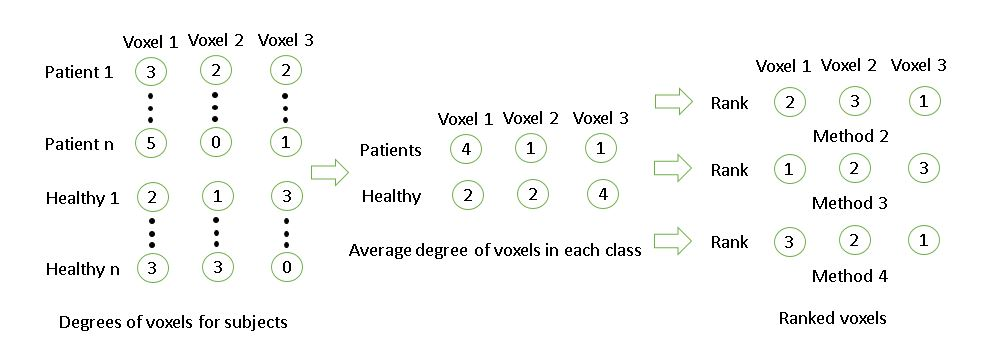
\includegraphics[width=\textwidth, height=4.5cm]{diagrams/Voxel_ranking.jpg}
\caption{Voxel ranking methods to select best voxels. In step 2, the differences of the average degrees between patients and healthy subjects are $2$, $-1$, and $-3$ respectively for the three voxels.}
\label{fig:voxel_rank_img}
\end{figure}
First, we executed the approach proposed by Rish \emph{et al.}~\cite{Rish_2013} 
on our data set. We had degrees of each voxels as well 
as the smoothed log values of the voxels for each subject. Furthermore, as 
some voxels of some subjects had zero values for the BOLD signal, an universal 
mask was used to select the voxels which had a non-zero BOLD signal value 
through the whole data set. This resulted in a $28719$ voxels per each subject. 
However, using all the available voxels resulted in significantly increased 
computation time
and thus selecting the best voxels (based on the training data) to separate 
the healthy and schizophrenic subjects was very important. 

To select the best voxels out of the possible $28719$ voxels, we experimented
with multiple approaches. These included selecting voxels based on t-tests, 
based on absolute differences of mean voxel degrees,
based on differences of mean voxel degrees ($schizophrenic - healthy$) and
based on differences of mean voxel degrees ($healthy - schizophrenic$).

%These included: \begin{enumerate}
%  \item Selecting voxels based on t-tests.
%  \item Selecting voxels based on absolute differences of mean degrees of a voxel between schizophrenic and healthy subjects.
%  \item Selecting voxels based on differences of mean degrees of a voxel between schizophrenic and healthy subjects.
%  \item Selecting voxels based on differences of mean degrees of a voxel between healthy and schizophrenic subjects.
%\end{enumerate}
The last three voxel ranking methods are explained in Figure~\ref{fig:voxel_rank_img}. 
Out of the above four approaches we obtained the highest accuracy on our cross 
validation set by the third approach. Also the number of voxels $k$ to be used 
in the SGMRF model was decided by running the experiment for different $k$ 
values and finding that $k = 20$ performed well during cross validation. By using the selected voxels, we obtained the precision matrices for schizophrenic and healthy subjects. Similar to the value of $k$, the sparsity coefficient 
$\lambda$ was also obtained through a hyper parameter search on our cross 
validation set.


\subsection{SGMRF with degrees from Dorsolateral Prefrontal Cortex area}
Connections in certain areas of the brain specifically dorsolateral 
prefrontal cortex (DLPFC)~\cite{Potkin2008} and 
thalamocortical~\cite{Cheng2015} circuitry. Thus, we extracted the degrees 
of voxels in these areas and used them to build the SGMRF model. Since we 
had only $4504$ voxels for each subject, we did not perform any voxel 
rankings in this approach. Similar to the previous approach using the 
smoothed log values of the degrees resulted in higher accuracy.

\subsection{Methods using Power \emph{et al.}'s ROIs}

The following three methods used in this subsection all involve the $264$  
regions of interest that are described in work by Power \emph{et al.}.
Due to missing data resulting from incomplete scans of subjects, $8$
regions were removed from analysis leaving $256$ ROIs. See appendix for
list of omitted region coordinates. We use the
approach described by Vega \emph{et al.}~\cite{rvega} to summarize
regions of interest by taking region averages for each of the $5mm$ radius
spheres that define regions. Finally this resulted in a $137 \times 256$ matrix
for each subject where each row is a time point across all regions and each
column is the average time series for a single region. The permitted SGMRF 
hyperparameter $\lambda$ values were $0.7$, $0.1$, $0.07$, $0.01$ and 
$0.007$ for this section.


\subsubsection{ROI with Subject Concatenation}

For this approach we follow the method described by Vega \emph{et al.}~\cite{rvega}.
Training set subjects in each class are first concatenated so that two large 
matrices are created, one with dimension $ns * 137 \times 256$ and the other 
with dimension $nh * 137 \times 256$ where $ns$ is the number of schizophenic 
subjects in the training set and $nh$ is the number of health subjects. To
make learning the SGMRF structure faster we also used the same feature 
normalization as was described by Vega \emph{et al.}~\cite{rvega},
where for each class and each region in that class the region mean was 
subtracted from each time point and each time point was divided by the 
region standard deviation. Next, with the use of Glasso, a SGMRF structure was 
learned for each class which resulted in two sparse precision matrices that 
encode the independences learned. Finally, when presented with a new subject 
from the hold-out set, equations \eqref{loglikelihood} and 
\eqref{logmaxlikelihood} were used to determine the likelihood of the subject 
belonging to each class followed by which class the new subject should be 
assigned.

A modified version of this approach was also implemented and tested but has
been omitted for brevity and due to it obtaining poor results.See appendix
for background information. In this variant,
a Fourier transform was used on each of the subject's time series data to 
obtain Fourier coefficients. These Fourier coefficients were then used in 
place of the original time series for learning a classifier.


\subsubsection{Region Degrees}

Like the work described in Rish \emph{et al.}~\cite{rish2009discriminative}, 
region degrees are also used in this approach but in this case, we only 
considered the degrees that result from the $256$ ROIs. This process is 
illustrated in Figure~\ref{fig:degree_calc}. The only difference in the
process described previously is that we explicitly remove the self 
correlations in the correlation matrix (the diagonal), and we conceptually
represent the process as binarizing a matrix and summing over its rows.
We also chose to use a threshold value of $0.7$ as was done in Rish 
\emph{et al.}~\cite{rish2009discriminative}.

\begin{figure}[!htb]
  \centering
  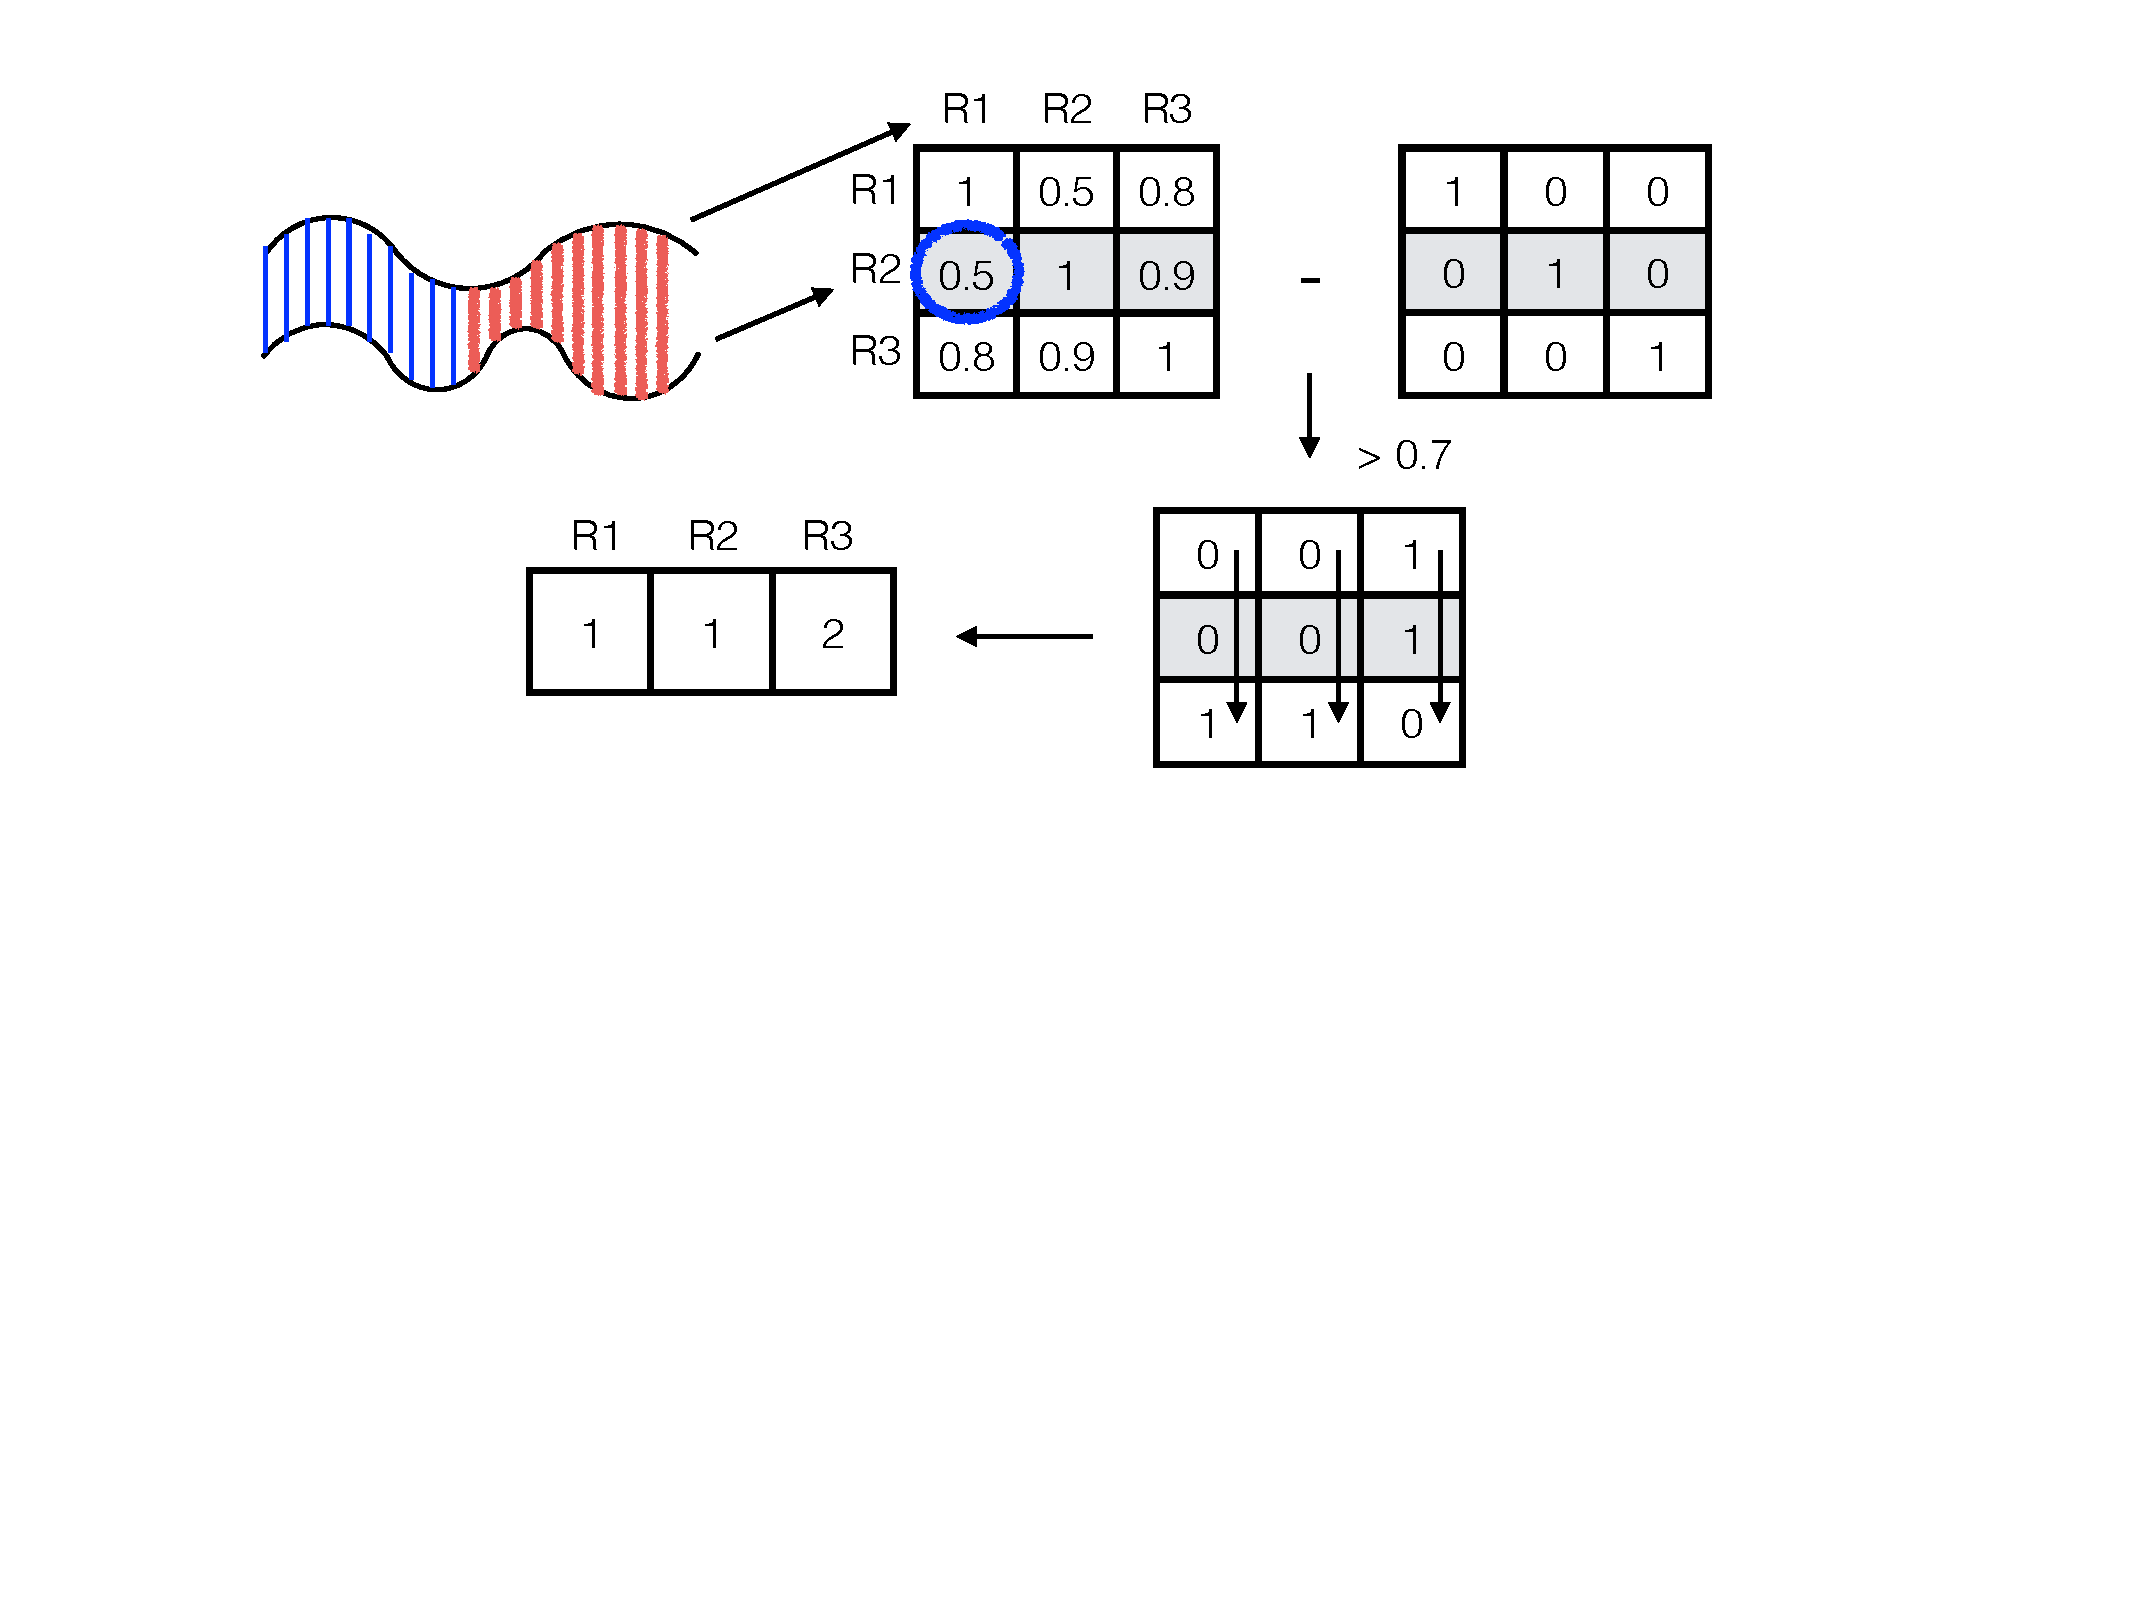
\includegraphics[width=0.7\textwidth, height=4.0cm]{diagrams/ROI_deg_img.pdf}
  \caption{Pair-wise comparisons are made between region time series data to
  produce a correlation matrix. The diagonal is removed and a threshold is
  applied to binarize the matrix. Sums are collected for each region to
  produce the ``degree'' of that region.}
  \label{fig:degree_calc}
\end{figure}

Now that we had a vector of region degrees ($1 \times 256$) for each subject,
a SGMRF was used to again to build a classifier. This followed similarly from
the previous approach except that now the input to Glasso was a $ns \times 256$
matrix for schizophrenic patients and a $nh \times256$ matrix for healthy
subjects. Again this resulted in two $256 \times 256$ precision matrices which
we could use in likelihood calculations for subjects from the hold-out set.
Additionally, we also used a linear SVM classifier trained directly on
region degree data to compare its performance to the SGMRF classifier.


\subsubsection{Individual MRF Structure Classification}

This approach is similar to the region concatenation approach described 
previously except that here we did not concatenate subjects and instead
learned a precision matrix (SGMRF structure) for each subject 
individually. For example, if we had $ns_{total}$ schizophrenics in our 
dataset and $nh_{total}$ healthy subjects ($ns_{total} + nh_{total}$ 
$137 \times 256$ matrices) then we would use Glasso to generate $ns + nh$ 
precision matrices.

To build a classifier, a linear SVM is trained on the precision matrices 
generated from the training set and then tested on the precision matrices 
generated from the hold-out set.

\subsection{Other Features Including PCA}
We have tried different features using the approach proposed by Rish \emph{et al.}. Features that are used for this approach are as following: [ Correlation , Log-Disconnection, Log-Disconnection Regions, Eignevalues, MBI stat, Degree].
This features were provided to us with the dataset. So we wanted to see how good results would be implementing the exact same approach as suggested by Rish \emph{et al.}. In this experiment we first selected the hyper parameters; number of features and $\lambda$; using $5$-fold cross validation and then test those parameters on the hold-out set. The hold-out set has been selected randomly from different site with criteria of being balanced with regards to healthy and schizophrenic, and according to the ratio of each group's subjects in each site. Result that we achieved had accuracy of less than 50\% for all features except than degrees and disconnection which achieved 65.55\% and 63.33\% accuracy respectively. 

Another approach that we have used for feature selection was using PCA for transforming the dataset to lower dimension. We hoped this could magnify distinguishing features in the dataset while reducing it size. Unfortunately results were not as we hoped and were mostly near the chance level. It should be mentioned that we chose three different sizes for the number of principal components that we used :3, 35 and 70.   


\section{Results and Discussion}

\begin{table*}[hpt]\footnotesize
\begin{center}
    \begin{tabular}{| l | r | r | r | r | r | r |}
    \hline
                & Rish (Full) & Rish (DLPFC) & ROI + Concatenation & Region Degrees & MRF structure & Other Features \\ \hline
    Classifier  & SGMRF       & SGMRF        & SGMRF               & SVM            & SVM           & SGMRF          \\ \hline
    Accuracy    & 72.32\%     & 63.52\%      & 74.17\%             & 60.65\%        & 69.44\%       & 65.55\%        \\ \hline
    \end{tabular}
    \caption{Accuracy on 5 Striated Hold-out Sets}
     \label{fig:holdout_table}
\end{center}
\end{table*}

As Seen in Table~\ref{fig:holdout_table} methods using a SGMRF classifier were
able to obtain the best results, of which $74.17\%$ was the highest average
accuracy recorded. This seems to suggest that a SGMRF seems to be a more
effective tool for this particular problem. A possible explanation for the
success of the SGMRF approach when using ROI and concatenating patient
data might be the results of reduced feature set size and increased input data
size for training. When comparing Rish (Full/DLPFC) in Table~\ref{fig:holdout_table} 
to the ROI $+$ Concatenation approach, the Rish approaches use voxels as their
features whereas ROI $+$ Concatenation only uses $256$ regions of interest as 
features. Given that our dataset only consists of $380$ examples, there is a 
much larger gap ($28719$ features for Full and $4504$ features for DLPFC) in 
number of features compared to number of training examples for these Rish 
approaches. Further, because each time point in the ROI $+$ Concatenation 
approach is considered as a sample from the region of interest, this approach
has $137$ times as much input data when training as compared to all other
methods used and it could be this that is boosting classification accuracy.
Between the two Rish methods we can see that DLPFC performs significantly
more poorly as compared to the other method which seems to suggest that the
DLPFC region is not sufficient for capturing the differences between controls
and schizophrenic patients. The region degrees approach also performed poorly.
While it is not clear why it performed so poorly, it might be the case that
voxel degree approaches need the full set of voxels to be effective. This would
explain the decreasing accuracies as we reduce the number of features used where
$28719$, $4504$ and $256$ features correspond to Rish (Full), Rish (DLPFC) and 
Region degrees, the voxel degree approaches tested. The approach classifying
subjects by the SGMRF structures learned performed surprisingly well which
suggests that a graphical models structure could potentially be useful, in 
addition to maximum likelihood when diagnosing schizophrenia. Finally, while
we considered many other features including PCA in our Other Features section, few performed
well. The best of these was closely related to the Rish (Full) approach which
indicated that voxel degrees have more discriminative power for this task as
compared to many other features.


\section{Conclusions and Future Work}
In this work we studied the use of fMRI and machine learning to diagnose
schizophrenia, given a set of healthy and schizophrenic subjects. We found
that a region based approach using SGMRFs yielded the highest accuracy 
($74.16\%$) when averaged over 5 hold-out sets where the hold-out set was
composed of $20\%$ of each site used in the study. We conclude from this
that ROIs are more effective in the diagnosis of schizophrenia then whole
brain analysis because extraneous noise is being removed from the data and
further, that representing your data in such a way to maximize the number
of training examples seen is beneficial to this problem.

In this study we did not select the number of principal components based 
on the variance captured by the components, future work could be done
to explore this method and determine if it could improve classification
accuracy. Other future work involves the use of ensemble methods. We have
found that several methods perform well individually, so an attempt at
combining them together seems like a natural next step.

\section{Acknowledgements}
We would like to thank Dr. Mina Gheiratmand for preprocessing the fMRI data 
and co-coaching our project, Sugai Liang for her advice and Roberto Vega for
all his advice and help. Finally, we would also like to thank Dr. Irina Rish
for the feature extraction code she provided and Dr. Greiner for his
supervision of this project.

\bibliographystyle{plain}
\bibliography{T4_Report}

\section{Appendix}

\subsection{Fourier Transform}
A Fourier transform allows for the translation of any signal from the time
domain to the frequency domain. More specifically, it takes a signal and
decomposes it into a series constituent $\sin$ and $\cos$ componets. When 
taking the Fast Fourier Transform or FFT of real data the resulting peaks in 
the frequency domain are conjugate symmetric~\cite{duhamel1990fast}, meaning 
that methods that only require the real component of the data need only work 
with half of the resulting component coefficients in the transform. These 
Fourier coefficients can be used in place of the original signal as features
provided to a machine learning classifier.

\subsection{Omitted ROI coordinates}
The regions removed
are characterized by region number with the associated MNI coordinates 
described in Power \emph{et al.} provided in parenthesis: 81 (-44, 12, -34), 
82 (46, 16, -30), 128 (52, 7, -30), 184 (17, -80, -34), 247 (33, 12, -34), 
248 (-31, -10, -36), 249 (49, -3, -38) and 250 (-50, -7, -39).

\subsection{Inference}
Once we have constructed probabilistic graphical model through precision 
matrix we can use that to do probabilistic inference for variables of 
interest. To make it more clear let assume $X$ is our dataset and 
$Z \subset X$ is the subset of our dataset which is observed with 
assigned values of $z$, and let $Y \subseteq X - Z$ be the set of unobserved 
variables. Now we can use inference to compute posterior probability of 
$P(Y|Z=z)$. In this task Y is a binary variable, and classification task is 
to find the assignment for y which makes the $P(Y|Z=z)$ maximum. 
$y^* = argmax_{y} P(Y=y|Z=z)$. Bayes rule give us: 

\begin{equation}
P(Y=y|Z=z) = \frac{P(Z=z|Y=y)P(Y=y)}{P(Z=z)}
\end{equation}  

And since denominator is fixed for each assignment Y=y. We compute the $argmax$ only using the numerator. 

\begin{equation}\label{argmax}
y^* = \argmax_{y} P(Z=z|Y=y)P(Y=y) 
\end{equation} 

So for a given dataset we can learn the model $ P(Z=z|Y=y)P(Y=y)$ for each 
class label, and then given a test dataset assign the most likely class 
label using the equation\eqref{argmax} \cite{Rish2014Book}  

\subsection{Description of the features }
\begin{enumerate}


\item Correlation: All pair-wise correlations between super-voxels in the (spatially) down-sampled data. The original data is 53x64x37 voxels. The number of all pair-wise correlations is extremely large for the original data. Data have been down sampled to 13x16x12. Then all of the pair-wise correlations computed, which is $(731x731-731)/2$. $731$ is the number of nonzero elements in the subjects universal brain mask (intersection of all subjects brains) in the down sampled data.

\item Eigenvalues: (Nonzero) eigenvalues of the correlation matrix

\item Log-disconnection: instead of thresholding for correlation coefficient $r > 0.7$ and finding the degrees, It has been thresholded for $r <0.4$ to have a measure of dis-connectivity of a voxel. In contrast, with the degree features. 

\item Log-disconnection regions: as the log-disconnection feature, but with only difference of being limited to three regions: superior frontal gyrus, middle frontal gyrus and Thalamus.  

\item MBI stat: statistics of the average brain intensity signal (for each subject) as the feature. These were mean, standard deviation, skewness and Kurtosis.

\item Degree: as described in the report.
\end{enumerate}
\end{document}
